\subsection{Der Map-Editor}
Ein weiteres Ziel dieses Projekts ist das Implementieren einer Applikation, die das Entwerfen und Speichern der Spielfelder, inklusive Checkpunkte und Startpositionen, erleichtern soll. Diese Applikation wird im Folgenden als Map-Editor bezeichnet.\\
In diesem Kapitel wird zunächst das Vorgehen der Erstellung eines Spielfeldes im Ausgangszustand des Rennspielframeworks geschildert. Anschließend wird auf das Konzept des Map-Editor eingegangen. Abschließend wird die Implementierung der Komponenten erläutert.\\

\subsubsection{Vorheriges Vorgehen bei der Spielfeld-Erstellung}
Da die Spielfelder mit ASCII-Zeichen kodiert werden und das Spielfeld hinzukommend eine festgelegte Größe von 20x30 Kacheln hat, ist das händische Erstellen einer solchen Datei ein aufwändiges Vorgehen. Hierbei besitzt jede Kachel eine eigene Identifikationsnummer. Ein Beispiel eines Spielfeldes und dessen Kodierung wird in \autoref{fig:simple_kodiert} dargestellt.\\

\begin{figure}[h]
\centering
\begin{minipage}{1.0\textwidth}
\centering
\begin{minipage}[t]{0.6\textwidth}
\centering
\begin{spacing}{1.0}
\fontsmall
MAP\\
10 10 10 10 10 10 10 10 10 10 10 10 10 10 10 10 10 10 10 10 10 10 10 10 10 10 10 10 10 10\\
10 20 20 20 20 20 20 20 20 20 20 20 20 20 20 20 20 20 20 20 20 20 20 20 20 20 20 20 20 10\\
10 20 21 18 18 18 18 18 18 18 18 18 18 18 18 18 18 18 18 18 18 18 18 18 18 18 18 22 20 10\\
10 20 16 11 11 11 11 11 11 11 11 11 11 11 11 11 11 11 11 11 11 11 11 11 11 11 11 15 20 10\\
10 20 16 11 11 11 11 11 11 11 11 11 11 11 11 11 11 11 11 11 11 11 11 11 11 11 11 15 20 10\\
10 20 16 11 11 12 13 13 13 13 13 13 13 13 13 13 13 13 13 13 13 13 13 13 14 11 11 15 20 10\\
10 20 16 11 11 15 20 20 20 20 20 20 20 20 20 20 20 20 20 20 20 20 20 20 16 11 11 15 20 10\\
10 20 16 11 11 15 20 20 20 20 20 20 20 20 20 20 20 20 20 20 20 20 20 20 16 11 11 15 20 10\\
10 20 16 11 11 15 20 20 20 20 20 20 31 32 32 32 33 20 20 20 20 20 20 20 16 11 11 15 20 10\\
10 20 16 11 11 15 20 20 20 20 20 20 34 30 30 30 35 20 20 20 20 20 20 20 16 11 11 15 20 10\\
10 20 16 11 11 15 20 20 20 20 20 20 36 37 37 37 38 20 20 20 20 20 20 20 16 11 11 15 20 10\\
10 20 16 11 11 15 20 20 20 20 20 20 20 20 20 20 20 20 20 20 20 20 20 20 16 11 11 15 20 10\\
10 20 16 11 11 15 20 20 20 20 20 20 20 20 20 20 20 20 20 20 20 20 20 20 16 11 11 15 20 10\\
10 20 16 11 11 15 20 20 20 20 20 20 20 20 20 20 20 20 20 20 20 20 20 20 16 11 11 15 20 10\\
10 20 16 11 11 17 18 18 18 46 18 18 18 18 18 18 18 18 18 18 18 18 18 18 19 11 11 15 20 10\\
10 20 16 11 11 11 11 11 11 45 09 09 11 11 11 11 11 11 11 11 11 11 11 11 11 11 11 15 20 10\\
10 20 16 11 11 11 11 11 11 45 09 09 11 11 11 11 11 11 11 11 11 11 11 11 11 11 11 15 20 10\\
10 20 23 13 13 13 13 13 13 47 13 13 13 13 13 13 13 13 13 13 13 13 13 13 13 13 13 24 20 10\\
10 20 20 20 20 20 20 20 20 20 20 20 20 20 20 20 20 20 20 20 20 20 20 20 20 20 20 20 20 10\\
10 10 10 10 10 10 10 10 10 10 10 10 10 10 10 10 10 10 10 10 10 10 10 10 10 10 10 10 10 10\\
\fontnormal
\end{spacing}
\label{fig:map_in_ascii}
\end{minipage}
\qquad
\begin{minipage}[t]{0.2\textwidth}
\begin{spacing}{1.0}
\fontsmall
CHECKPOINT\\
07 16 01\\
07 17 01\\
04 14 02\\ 
05 14 02\\
04 07 03\\
05 07 03\\
08 04 04\\
08 05 04\\
23 04 05\\
23 05 05\\
26 08 06\\
27 08 06\\
26 14 07\\
27 14 07\\
STARTPOINT\\
10 15 3\\
10 16 3\\
11 15 3\\
 11 16 3\\


\end{spacing}
\fontnormal
%\subcaption{Kodierung der Check- und Startpositionen}
\end{minipage}
\subcaption{Kodierung des Spielfeldes mit Checkpunkten und Startpositionen}
\end{minipage}
\begin{minipage} {0.9\textwidth}
\centering
\includegraphics[scale=0.25]{pics/simples_spielfeld.png}
\label{fig:check_start}
\subcaption{Ergebnis der obigen Kodierung}
\end{minipage}
\caption{Beispielhaftes Spielfeld mit der dazugehörigen Kodierung}
\label{fig:simple_kodiert}
\end{figure}

Hinzukommend müssen die Positionen für die Start- und Checkpunkte (siehe \autoref{fig:check_start}) angegeben werden. Damit diese und weitere Informationen für ein Spiel verwendet werden können, müssen diese in einer JSON-Konfigurationsdatei abschließend angegeben werden. Anhand dieses Beispiels ist gut zu erkennen, dass das Erstellen eines Spielfeldes einen aufwändigen Prozess darstellen kann.\\
Der Map-Editor soll dementsprechend folgende Anforderungen erfüllen:
\begin{itemize}
\item Das Erstellen des Spielfeldes soll dem Nutzer nicht nur via ASCII-Kodierung gelingen können.
\item Der Nutzer soll dazu in der Lage sein, Start- und Checkpunkte setzen zu können.
\item Das Spielfeld, dessen Start- und Checkpunkte sollen anschließend korrekt kodiert in einer Datei gespeichert werden.
\end{itemize}
Um die Umsetzung dieses Vorgehens und die Erweiterung neuer Funktionalitäten dem Entwickler zu erleichtern, orientiert sich die Architektur des Map-Editors an dem MVC-Architekturmuster (siehe Kapitel ???). Die Umsetzung der Architektur wird im folgenden Abschnitt genauer erläutert.

\subsubsection{Architektur des Map-Editors}
In der folgenden Abbildung werden die grundlegenden Komponenten des Editors in Form eines Domänenmodells dargestellt.\\

\begin{figure}[h]
\centering
\includegraphics[scale=0.5]{pics/mapeditor_domain.png}
\caption{Domänenmodell des Map-Editors}
\label{fig:domain_mapeditor}
\end{figure}

Das MVC-Muster ist hierbei wie folgt zu sehen:
\begin{itemize}
\item View wird durch die \texttt{GUI}-Komponenten dargestellt. Alle Aufgaben, die zur Ausgabe dienen, sind vereinfacht in dieser Komponente zusammengefasst. Der Übersichtlichkeit halber werden hier nicht alle Komponenten, die mit der Aktion des Anwenders zu tun haben dargestellt.
\item Controller wird durch die Komponenten \texttt{TileController} und \texttt{TableConverter} dargestellt. Zusätzlich befinden sich hier die Komponenten des Memento-Entwurfsmusters. Diese Komponenten werden der Einfachheit halber nicht dargestellt. Eine nähere Erläuterung der Umsetzung dieses Musters erfolgt im kommenden Abschnitt.
\item Model wird durch \texttt{TileReader} dargestellt. Diese Komponente übernimmt alle E/A-Aufgaben, wozu das Einlesen und Erstellen von Konfigurationsdateien des Spielfeldes zählen.
\end{itemize}
Dieses Architekturmuster hilft hierbei eine eindeutige Trennung der Komponenten und deren Funktionalität zu schaffen. Wird nun beispielsweise aus der \texttt{Gui} das Speichern des aktuellen Spielfeldes gestartet, so erfolgt eine Verbindung zur Model-Schicht mittels des \texttt{TileControllers}, damit für eine zusätzliche klare Trennung der Schichten gesorgt werden kann. Dementsprechend fungiert der \texttt{TileController} als Hauptansprechpartner, falls eine Aktion aus der \texttt{Gui} heraus gestartet wird. Dies bringt zwar eine niedrige Kohäsion mit sich, da die \textit{TileController}-Komponente für sowohl das Speichern von Dateien, als auch für das Ausführen der Logik der \textit{Gui}-Aktionen zuständig ist. Dies hat jedoch bei den überschaubaren Funktionalitäten des Map-Editors, die im kommenden Abschnitt genauer beschrieben werden, eine geringe Auswirkung.\\
Die Implementierung der Komponenten und zusätzliche Eigenschaften des Map-Editors werden im folgenden Unterabschnitt erläutert, wobei zunächst auf die Funktionalität und den Ablauf des Erstellen eines Spielfeldes eingegangen wird.

\subsubsection{Implementierung des Map-Editors}
Wie in \autoref{fig:layout-mapeditor} zu sehen ist, besteht die grafische Oberfläche des Map-Editors aus drei Label, in denen sich eine Auswahl möglicher Kacheln (links), das aktuelle Spielfeld in Form einer Tabelle (rechts oben) und eine Auswahl der möglichen Befehle, die der Nutzer zur Bearbeitung des Spielfelds verwenden kann, in Form von Buttons (unten).

\begin{figure} [h]
\centering
\includegraphics[scale=0.45]{pics/map-editor-layout.png}
\caption{Grafische Oberfläche des Map-Editors}
\label{fig:layout-mapeditor}
\end{figure}

Für die Auswahl möglicher Kacheln werden diese Daten aus einer Konfigurationsdatei erfasst. Diese Aufgabe übernimmt die Komponente \texttt{TileReader} aus der Model-Komponente. Es werden hierbei zuerst alle möglichen Kacheln mit deren IDs eingelesen. Anschließend werden die Bilder dieser Kacheln eingelesen. Jedes Kachelbild wird mit der korrespondierenden ID der Kachel in einem Label gespeichert. Anschließend wird nur das Bild als visuelle Ausgabe des Labels dargestellt. Jedes Label hat also das Kachel-Bild und die korrespondierende ID gespeichert. Die ID ist hierbei notwendig, um abschließend aus der Tabelle eine Konfigurationsdatei des Spielfeldes in ASCII-Form abspeichern zu können.\\
Die Tabelle rechts in \autoref{fig:layout-mapeditor} dient, wie bereits beschrieben, dem Erstellen der Spielfelder. Die Tabelle zeigt hierbei nur das Bild der Kachel an. Zusätzlich wird in jeder Zelle der Tabelle die dazugehörige ID zur Kachel abgespeichert, damit das Speichern des Spielfeldes zusätzlich erleichtert wird.\\
Was den Vorgang des Erstellen des Feldes betrifft, so soll der Anwender die gewünschte Kachel aus dem Auswahlmenü in die jeweilige Zelle der Tabelle ziehen. Falls mehrere Zellen auf einmal befüllt werden sollen, so kann ein Bereich markiert werden. Wird in diesem Bereich eine Kachel reingezogen, so wird der ausgewählte Bereich auf einmal überschrieben. Dies hat die Intention, dem Anwender das Erstellen der Spielfelder zu erleichtern und zusätzlich den gesamten Ablauf zu verkürzen. Der Rand des Spielfeldes wird hierbei standardsgemäß mit der Mauer-Kachel gefüllt und kann nicht von anderen Kacheln überschrieben werden. Dies ist notwendig, damit die Spieler nicht aus dem Spielfeld hinaus fahren können.\\
Sind Zellen noch nicht überschrieben worden, stellen diese also eine leere Zelle dar, so wird für diese Zellen die Kachel-ID -1 verwendet und ein weißes Bild zur Ausgabe verwendet. Stellt eine Zelle einen Start- oder Checkpunkt dar, so werden die Bilder dieser Zellen aufgehellt, um dem Anwender dies zu visualisieren.\\
Weitere Funktionalitäten des Map-Editors und deren Implementierung lauten wie folgt:

\textbf{Das Füllen aller leeren Zellen der Tabelle mit Grass}\\
Hierbei wird über den gesamten Tabelleninhalt iteriert und die Zellen, die aktuell noch mit der ID -1 gefüllt sind, mit den Grass-Tiles überschrieben. So kann sich der Anwender auf das Erstellen der Strukturen der Rennstrecken fokussieren und die Zeit zum Erstellen eines Spielfeldes wird zusätzlich reduziert.

\textbf{Das Erstellen von Startpositionen und Checkpunkten}\\
Hierfür muss mindestens eine Zelle der Tabelle ausgewählt sein. Der Nutzer wird anschließend nach der Positionierungsrichtung der Fahrzeuge gefragt. Die Koordinaten und die angegebene Richtung werden anschließend gespeichert. Werden neue Startpositionen ausgewählt, so werden diese standardsgemäß zu den aktuell gespeicherten Startpositionen hinzugefügt. Das Setzen der Checkpunkte erfolgt analog zu den Startpunkten, jedoch ohne der Auswahl der zu fahrenden Richtung der Spieler. Auch hier werden neu gesetzten Checkpunkte zu den aktuell gespeicherten Punkten hinzugefügt.

\textbf{Das Löschen der Start- und Checkpunkte}\\
Der Nutzer kann alle bereits gesetzten Startpunkte löschen. Hierbei werden lediglich die gespeicherten Startpunkte auf den Initialwert zurückgesetzt. Das Löschen aller Checkpunkte erfolgt hierzu erneut analog.

\textbf{Bereits erstellte Spielfelder einlesen}\\
Um bereits erstelle Spielfelder überarbeiten zu können, kann der Anwender die zu überarbeitende Datei in einem Auswahlmenü selektieren. Anschließend werden diese Datei eingelesen. Die Tabelle wird abschließend komplett überschrieben, so dass diese der eingelesenen Informationen ähnelt.

\textbf{Das Füllen eines Bereichs der Tabelle}\\
Wie bereits erwähnt, können mehrere Felder gleichzeitig befüllt werden. Hierzu kann der Nutzer einen beliebigen Bereich der Tabelle auswählen und anschließend eine beliebige Kachel auf eines der markierten Felder ziehen. Bei diesem Vorgang wird zunächst überprüft, ob mehrere Zellen ausgewählt wurden. Ist dies der Fall, so werden alle betroffenen Zellen überschrieben.

\textbf{Das Visualisieren des markierten Bereichs und der Start- und Checkpunkte}\\
Damit der markierte Bereich dem Anwender visuell dargestellt werden kann und der Anwender somit eine Rückmeldung des Programms bekommt, wird bei jedem Aktualisieren der Tabelle das Bild der markierten Zelle heller abgespeichert (siehe \autoref{fig:layout-mapeditor}). Ist eine Zelle nicht mehr markiert, so wird auf das originale Kachel-Bild zurückgesetzt. Dieser Mechanismus wird auch bei den Startpositionen und Checkpunkten verwendet, damit diese dem Anwender deutlich dargestellt werden können. Hierbei werden die Startpositionen dunkler und die Checkpunkte heller dargestellt, wie in \autoref{fig:layout-mapeditor} zu sehen ist.

\textbf{Die Grenzen des Spielfelds werden nie überschrieben}\\
Damit die Grenzen des Spielfeldes immer vorhanden sind, ist der Rand der Tabelle immer mit einer Mauer-Kachel belegt. Versucht der Anwender trotzdem eines dieser Felder zu überschreiben, so wird dieser Befehl ignoriert. Dem Nutzer wird anschließend eine Warnmeldung ausgegebene. Die Überprüfung, ob ein Rand-Element überschrieben wird, erfolgt auch bei einer Mehrfachauswahl von Tabellen-Zellen.

\textbf{Das Speichern des Spielfeldes}\\
Beim Speichern des Spielfeldes und der zugehörigen Informationen wird zunächst überprüft, ob alle Zellen der Tabelle mit bekannten Tile-IDs gefüllt sind, mindestens ein Chechpunkt und mindestens ein Startpunkt gesetzt sind. Ist mindestens eine dieser Bedingungen nicht erfüllt, so wird zunächst eine Warnung, dass der Stand des Spielfeldes noch kein akzeptiertes Feld darstellt, ausgegeben. Anschließend kann der Anwender entweder abbrechen oder den aktuellen Stand trotzdem speichern, falls lediglich ein Zwischenstand gesichert werden soll. Bei dem Erstellen der Datei des Spielfeldes wird über den Tabelleninhalt iteriert und die Kachel-IDs werden wie in \autoref{fig:check_start} zeilenweise angeordnet und in eine neue Datei geschrieben. Die Check- und Startpunkte werden in derselben Datei gespeichert. Damit eine eindeutige Unterscheidung der verschiedenen Sektionen erfolgen kann, wird in die vorherige Zeile des jeweiligen Abschnitts ein Name geschrieben, der die dazugehörige Komponente bezeichnet. Den Namen der produzierten Konfigurationsdatei hat der Anwender zu Beginn des Vorgangs angegeben.

\textbf{Gemachte Aktionen rückgängig machen}\\
Des Weiteren kann der Anwender seine zuletzt durchgeführten Aktionen rückgängig machen. Die Umsetzung hierbei erfolgt über das Memento-Muster \textbf{(siehe Kapitel ??)}. Hierbei wird für den aktuellen Zustand der Inhalt der Tabelle, die gesetzten Startpunkte und die gesetzten Checkpunkte verwendet. Ein Zustand wird als Memento gespeichert, sofern sich der Tabelleninhalt, die Start- oder Checkpunkte verändern. Wird nun ein vorheriger Zustand geladen, so werden auch diese Informationen komplett überschrieben und die Tabelle wird zur Visualisierung aktualisiert. Das Memento-Muster ist hierbei wie folgt umgesetzt:

\begin{figure}[h]
\centering
\begin{tikzpicture}
\tikzumlset{fill class = white, fill template = white}
	\umlclass[x=0]{Originator}{ - karte \\ - startpunkte \\ - checkpunkte \\ - letzterSicherungspunkt \\ - caretaker }{ + erstelleSicherung()\\ + undo() \\ + restore() \\ + setOriginatorZustand(ID) }
	\umlclass[x=5.5]{Memento} { - katze \\ - startpunkte \\ - checkpunkte }{ + SetZustand() }
	\umlclass [x=11.3] {Caretaker}{ - zustände \\ - mementoID}{ + speichereMemento() \\ + getMemento(ID)}

	
	\umlimport[]{Originator}{Memento};
	\umluniaggreg[arg=memento, pos=0.5]{Caretaker}{Memento};
	%\umlnote[y=-3, width=4cm, fill=white]{Kontext}{ruft auf:\\ strategie.algorithmus()}

\end{tikzpicture}
\caption{Umsetzung des Memento-Musters für den Map-Editor}
\label{fig:memento_imp}
\end{figure}

\begin{itemize}
\item Wie in \autoref{fig:memento_imp} zu sehen ist, besitzt die \textit{Memento-Klasse}, die die gespeicherten Zustände darstellt, Attribute für das Spielfeld, den Startpositionen und den Checkpunkten.
\item Der \textit{Originator}, der den aktuellen Zustand des Editors darstellt, besitzt zusätzlich den letzten Sicherungspunkt der vorherigen \textit{Memento}-Instanz.
\item Hinzukommend wird ein Verwalter, der \texttt{Caretaker}, für das Erstellen und Wiederherstellen der Zustände verwendet. Dieser hat alle erstellten \textit{Memento}-Instanzen mit einer ID in einer Hash-Map abgespeichert. Mit der Angabe der jeweiligen ID kann nun ein beliebiger Zustand wiederhergestellt werden. Dies ermöglicht auch in Zustände zu gelangen, die bereits erreicht wurden, falls der Anwender z.B. zu oft rückgängig gemacht hat und wieder ein paar Zustände nach vorne gelangen will. 
\end{itemize}
Wird nun die Tabelle verändert, so wird der aktuelle Zustand der Tabelle in den \texttt{Originator} geschrieben und zusätzlich ein Sicherungspunkt erstellt. Der \texttt{Originator} wird zusätzlich verändert, wenn ein Sicherungspunkt oder ein Startpunkt gesetzt wird. Setzt nun der Anwender einen vorherigen Stand zurück, so wird die jeweilige \texttt{Memento}-Instanz geladen und der Zustand des \texttt{Originators} überschrieben. Wie bereits beschrieben, hat anschließend der Nutzer die Möglichkeit wieder einen Zustand nach vorne zu springen. Hierbei ergibt sich der folgende Spezialfall:\\
Macht der Anwender seine Änderungen rückgängig und ändert die Tabelle, so soll dieser nicht mehr nach vorne springen können, da ansonsten die neue Änderung des Nutzers verloren gehen würde. Tritt also ein solcher Fall ein, so werden nach der Überschreibung des \texttt{Originators}, also beispielsweise nach Tabellenänderung, alle nachfolgenden \texttt{Memento}-Elemente gelöscht, damit keine Inkonsistenzen entstehen. \autoref{fig:memento_example} veranschaulicht diesen Mechanismus.\\ 

\begin{figure}[h]
\centering
\begin{minipage}[b]{0.3\textwidth}
\centering
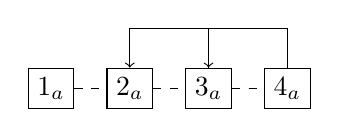
\begin{tikzpicture}
        \node at (0,0) [rectangle,draw] (a1) {$1_{a}$};
        \node at (1,0) [rectangle,draw] (a2) {$2_{a}$};
        \node at (2,0) [rectangle,draw] (a3) {$3_{a}$};
        \node at (3,0) [rectangle,draw] (a4) {$4_{a}$};
        \draw[->] (a4.north) -- ++(0,0.5) -- ++(-1,0) -- (a3.north);
        \draw[->] (a3.north) -- ++(0,0.5) -- ++(-1,0) -- (a2.north);
        \draw[-,dashed] (a1) -- (a2);
        \draw[-,dashed] (a2) -- (a3);
        \draw[-,dashed] (a3) -- (a4);
\end{tikzpicture}
\subcaption{Zwei Aktionen rückgängig}
\label{fig:memento_zweinachhinten}
\end{minipage}
\qquad
\begin{minipage}[b]{0.3\textwidth}
\centering
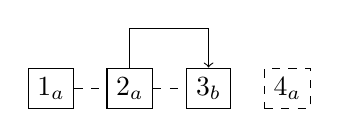
\begin{tikzpicture}
        \node at (0,0) [rectangle,draw] (a1) {$1_{a}$};
        \node at (1,0) [rectangle,draw] (a2) {$2_{a}$};
        \node at (2,0) [rectangle,draw] (a3) {$3_{b}$};
        \node at (3,0) [rectangle,draw,dashed] (a4) {$4_{a}$};
        \draw[->] (a2.north) -- ++(0,0.5) -- ++(1,0) -- (a3.north);
        \draw[-,dashed] (a1) -- (a2);
        \draw[-,dashed] (a2) -- (a3);
\end{tikzpicture}
\subcaption{Neue Aktion durchführen}
\label{fig:memento_überschreiben}
\end{minipage}
\qquad
\begin{minipage}[b]{0.25\textwidth}
\centering
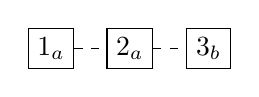
\begin{tikzpicture}
        \node at (0,0) [rectangle,draw] (a1) {$1_{a}$};
        \node at (1,0) [rectangle,draw] (a2) {$2_{a}$};
        \node at (2,0) [rectangle,draw] (a3) {$3_{b}$};
        \draw[-,dashed] (a1) -- (a2);
        \draw[-,dashed] (a2) -- (a3);
\end{tikzpicture}
\subcaption{Endergebnis}
\label{fig:memento_nachher}
\end{minipage}

\caption{Ablauf, wenn ein nicht aktueller Zustand überschrieben wird}
\label{fig:memento_example}
\end{figure}

Hier befindet sich der aktuelle Zustand des Systems bei $4_{a}$. Der Anwender macht die letzten zwei Aktionen rückgängig und gelangt in den Zustand $2_{a}$ (siehe \autoref{fig:memento_zweinachhinten}). Anschließend erfolgt eine Änderung durch den Nutzer, wodurch der Zustand $3_{a}$ durch $3_{b}$, welcher den neuen Zustand beinhaltet, überschrieben wird. Anschließend wird der Folgezustand $4_{a}$ entfernt, da dieser mit der neuen Zustandskette keinen Sinn ergibt. Würde $4_{a}$ nicht entfernt werden, so kann der Nutzer einen Zustand noch vorne springen, was mit der neu gemachten Aktion in $3_{b}$ nichts mehr zu tun hat. Somit sind nur die Zustände gespeichert, die in \autoref{fig:memento_nachher} zu sehen sind.







